\def\layersep{2.25cm}
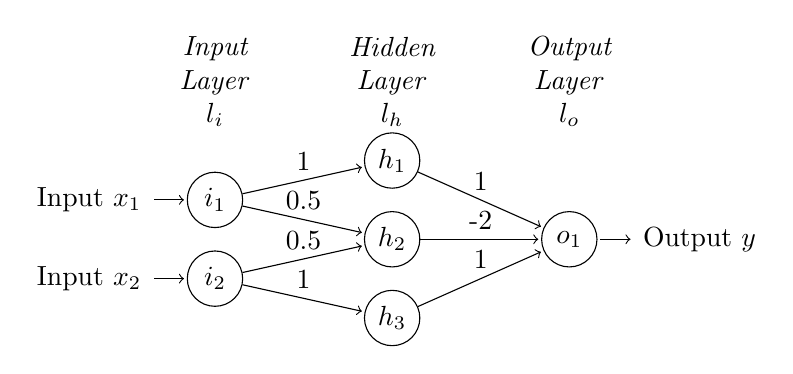
\begin{tikzpicture}[shorten >=1pt,->,draw=black!100, node distance=\layersep]
	\tikzstyle{every pin edge}=[<-,shorten <=1pt]
	\tikzstyle{neuron}=[circle,fill=black!25,minimum size=20pt,inner sep=0pt]
	\tikzstyle{input neuron}=[neuron, fill=white!100,draw=black];
	\tikzstyle{output neuron}=[neuron, fill=white!100,draw=black];
	\tikzstyle{hidden neuron}=[neuron, fill=white!100,draw=black];
	\tikzstyle{annot} = [text width=4em, text centered]
	
	% Draw the input layer nodes
	\foreach \name / \y in {1,...,2}
	% This is the same as writing \foreach \name / \y in {1/1,2/2,3/3,4/4}
	\node[input neuron, pin=left:Input $x_\y$] (I-\name) at (0,-\y) {$i_\y$};
	
	% Draw the hidden layer nodes
	\foreach \name / \y in {1,...,3}
	\path[yshift=0.5cm]
	node[hidden neuron] (H-\name) at (\layersep,-\y cm) {$h_\y$};
	
	% Draw the output layer node
	\node[output neuron,pin={[pin edge={->}]right:Output $y$}, right of=H-2] (O1) {$o_1$};
	
	% Connect every node in the input layer with every node in the
	% hidden layer.
	%\foreach \source in {1,...,2}
	%\foreach \dest in {1,...,3}
	%\path (I-\source) edge node[above] {1} (H-\dest);
	\path (I-1) edge node[above] {1} (H-1);
	\path (I-1) edge node[above] {0.5} (H-2);
	\path (I-2) edge node[above] {0.5} (H-2);
	\path (I-2) edge node[above] {1} (H-3);
	
	% Connect every node in the hidden layer with the output layer
	%\foreach \source in {1,...,3}
	\path (H-1) edge node[above] {1} (O1);
	\path (H-2) edge node[above] {-2} (O1);
	\path (H-3) edge node[above] {1} (O1);
	
	% Annotate the layers
	\node[annot,above of=H-1, node distance=1cm] (hl) {\textit{Hidden Layer}\\$l_h$};
	\node[annot,left of=hl] {\textit{Input Layer}\\$l_i$};
	\node[annot,right of=hl] {\textit{Output Layer}\\$l_o$};
\end{tikzpicture}